\chead{CHAPITRE 5 . SPRINT 3:  \textbf{Gestion des Entretiens et ATS}}

\chapter{Sprint 3: Gestion des Entretiens et ATS}
\renewcommand{\mtctitle}{Sommaire}
\minitoc
\newpage
\section*{Introduction}
\addcontentsline{toc}{section}{\protect\numberline{}Introduction}%
Ce chapitre explore les étapes de la Sprint Gestion des Entretiens et ATS, avec un accent particulier sur la gestion des processus d’entretien et l’utilisation d’un système ATS. Nous débuterons par un aperçu du backlog, avant de détailler la conception, la mise en œuvre et d’illustrer le travail effectué à l’aide de captures d’écran.
\section{Objectifs du Sprint}
L’objectif de cette sprint est de mettre en place un système ATS pour filtrer les CV, gérer les statuts des candidats, planifier et modifier les entretiens, ainsi qu’envoyer des mails automatiques.


\section{Spécification des besoins}
\par Dans cette section, nous allons débuter par présenter le diagramme de cas d’utilisation de la sprint, suivi de l’exposition du backlog associé.
\subsection{Diagramme cas d’utilisation du Sprint 3}


\begin{figure}[H]
\centering
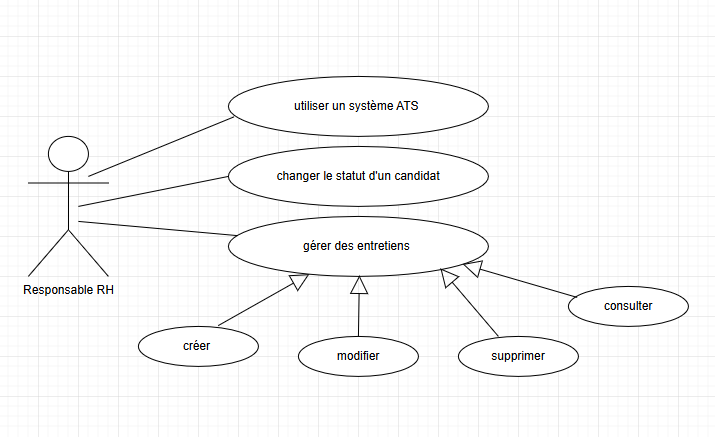
\includegraphics[width=18cm, height=9cm]{Figures/use case 3.png}
\caption{Diagramme cas d’utilisation du sprint 3}
\label{schema1}
\end{figure}


\subsection{ Sprint Backlog du sprint 3}
Le tableau suivant illustre le sprint backlog établi pour le troisième sprint. Il récapitule les différentes user stories sélectionnées, accompagnées de leurs identifiants uniques, ainsi que les tâches techniques à réaliser pour chacune. Ce tableau permet d’avoir une vision claire et structurée du travail prévu, en facilitant la planification, la répartition des responsabilités et le suivi de l’avancement tout au long du sprint.



\begin{table}[H]
\caption{Backlog du sprint 3}
\centering
\begin{tabular}{|p{1cm}|p{8cm}|p{8cm}|}
\hline
\textbf{ID} & \textbf{User Story} & \textbf{Tâches techniques} \\
\hline
US-13 & En tant que responsable RH, je veux utiliser un système ATS pour filtrer automatiquement les CV et prioriser les profils. 
& 
\begin{itemize}[leftmargin=*]
  \item Développer un algorithme de filtrage des CV.
  \item Implémenter un système de score/priorité.
  \item Créer l'interface de visualisation des résultats filtrés.
\end{itemize} \\
\hline
US-14 & En tant que responsable RH, je veux changer le statut d’un candidat. 
& 
\begin{itemize}[leftmargin=*]
  \item Ajouter un champ "statut" dans le modèle "Candidature".
  \item Connecter l’action à la base de données.
\end{itemize} \\
\hline
US-15 & En tant que responsable RH, je veux planifier des entretiens. 
& 
\begin{itemize}[leftmargin=*]
  \item Créer un formulaire de planification d’entretien.
\end{itemize} \\
\hline
US-16 & En tant que responsable RH, je veux modifier ou supprimer un entretien déjà planifié. 
& 
\begin{itemize}[leftmargin=*]
  \item Créer les options "modifier" et "supprimer" sur le calendrier.
  \item Gérer les mises à jour et suppressions côté base.
  \item Afficher les messages de confirmation.
\end{itemize} \\
\hline
\end{tabular}
\label{tab:sprint3_backlog}
\end{table}




\section{Analyse des besoins}
Avant de modéliser les fonctionnalités du système, il est essentiel de comprendre les besoins fonctionnels exprimés à travers les différents cas d’usage. La section suivante propose une description textuelle de ces cas d’utilisation, permettant de mieux cerner les interactions entre les utilisateurs et le système, et de poser les bases d’une modélisation cohérente. 
    
\subsection{Description textuelle de cas d'utilisation}

     \item \textbf{Cas d'utilisation "Utiliser un système ATS": } La table 5.2 ci-dessous présente la description textuelle du cas d'utilisation « Utiliser un système ATS ».

 \begin{table}[H]
 \caption{ Description textuelle du cas d’utilisation "Utiliser un système ATS"}
    \centering
    \begin{tabular}{|c|p{12cm}|}
    \hline
    \textbf{Titre} & Utiliser un système ATS \\
    \hline
    \textbf{Objectif} & Permettre au responsable RH d’utiliser un système ATS pour filtrer automatiquement les CV et prioriser les profils des candidats. \\
    \hline
    \textbf{Acteur}& Responsable RH\\
    \hline
    \textbf{Pré-condition} & Le responsable RH doit être authentifié et le système ATS doit être configuré.
    \\
    \hline
    \textbf{Post-condition} & Les CV sont filtrés et une liste de profils prioritaires est générée.\\
    \hline
    \textbf{Scénario nominal} & 1. Le responsable RH accède à l’interface de candidatures \newline
    2. Le système ATS filtre automatiquement les candidatures.\newline
    3. La liste des candidatures filtrées s’affiche directement.
    \newline
    4. Il consulte les résultats prioritaires.\\
    \hline
    \end{tabular}
    \label{tab:user_stories}
\end{table}


     \item \textbf{Cas d'utilisation "Changer le statut d'un candidat": } La table 5.3 ci-dessous présente la description textuelle du cas d'utilisation « Changer le statut d'un candidat ».

 \begin{table}[H]
 \caption{ Description textuelle du cas d’utilisation "Changer le statut d'un candidat"}
    \centering
    \begin{tabular}{|c|p{12cm}|}
    \hline
    \textbf{Titre} & Changer le statut d'un candidat \\
    \hline
    \textbf{Objectif} & Permettre au responsable RH de modifier le statut d’un candidat (en attente, entretien, accepté, refusé). \\
    \hline
    \textbf{Acteur}& Responsable RH\\
    \hline
    \textbf{Pré-condition} & Une candidature doit exister dans le système.
    \\
    \hline
    \textbf{Post-condition} & Le nouveau statut du candidat est mis à jour et visible.\\
    \hline
    \textbf{Scénario nominal} & 1. Le responsable RH accède à la gestion des entretiens. \newline
    2. Il planifie un entretien pour un candidat.\newline
    3. Le système change automatiquement le statut (ex. "En entretien").
    \newline
    4. Après l’entretien, il enregistre le résultat.
    5. Le système met à jour le statut automatiquement (ex. "Accepté" ou "Refusé").\\
    \hline
    \end{tabular}
    \label{tab:user_stories}
\end{table}

     \item \textbf{Cas d'utilisation "Gérer des entretiens": } La table 5.4 ci-dessous présente la description textuelle du cas d'utilisation « Gérer des entretiens ».

 \begin{table}[H]
 \caption{ Description textuelle du cas d’utilisation "Gérer des entretiens"}
    \centering
    \begin{tabular}{|c|p{12cm}|}
    \hline
    \textbf{Titre} & Gérer des entretiens \\
    \hline
    \textbf{Objectif} & Permettre au responsable RH de créer, modifier, supprimer et consulter les entretiens planifiés. \\
    \hline
    \textbf{Acteur}& Responsable RH\\
    \hline
    \textbf{Pré-condition} & Le responsable RH doit être authentifié et un candidat doit être sélectionné.
    \\
    \hline
    \textbf{Post-condition} & Les modifications ou suppressions des entretiens sont enregistrées dans le système.\\
    \hline
    \textbf{Scénario nominal} & 1. Le responsable RH accède à la gestion des entretiens. \newline
    2. Il sélectionne une action (créer, modifier, supprimer).\newline
    3. Il entre les détails (date, heure, candidat).
    \newline
    4. Le système valide et enregistre les données.\\
    \hline
    \end{tabular}
    \label{tab:user_stories}
\end{table}

\section{Conception}
\hspace{0.5cm}\textbf Dans cette section, nous discutons de la conception du troisème sprint. nous Commençons par le diagramme de classes du sprint. Ensuite, nous examinons la modélisation de quelques diagrammes de séquences. 





    \subsection{Diagrammes de séquences}
    Dans le cadre de l’analyse dynamique du système, un diagramme de séquence a été réalisé pour chaque fonctionnalité clé développée lors des sprints. Le diagramme ci-dessous illustre spécifiquement le scénario du cas d'utilisation « Gérer un entretien », permettant de visualiser les interactions entre le responsable rh et le système lors de la création d’un nouvel entretien.

    \subsubsection{Diagramme de séquence au cas d’utilisation «Gestion des données importées»}
Cette figure illustre le déroulement du scénario associé à ce cas d'utilisation.
     \begin{figure}[H]
    \centering
   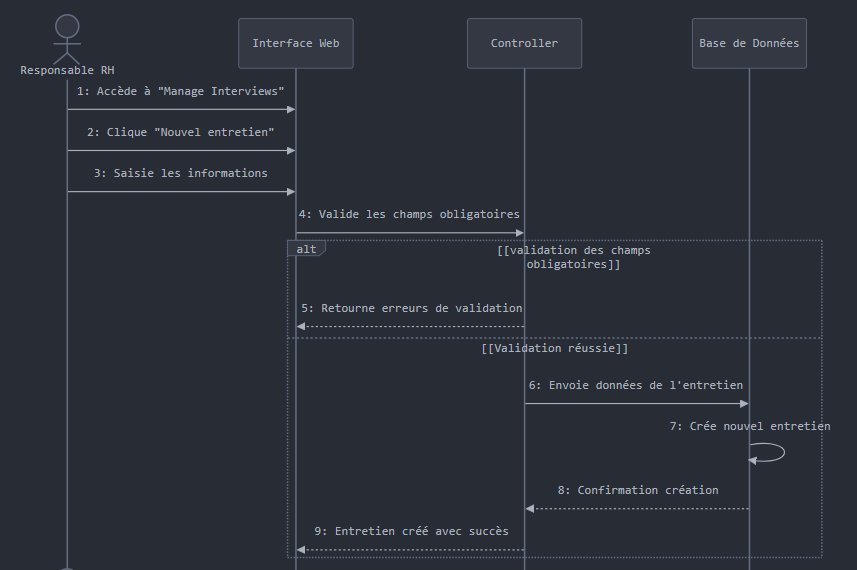
\includegraphics[width=18cm, height=18cm]{Figures/seq3.png}
    \caption{Diagramme de séquence détaillé  au scénario Gestion des entretiens»}

\end{figure}

\section{Réalisation: interfaces Utilisateur dans RhNova }
Dans ce qui suit, nous présentons l’interface dédiée à la gestion des entretiens, qui permet au responsable RH de planifier, modifier ou consulter les entretiens organisés avec les candidats de manière intuitive et structurée.


\vspace{5mm}
\begin{itemize}
     \begin{itemize}
      \item \textbf{Gestion des entretiens  : }Cette interface permet au responsable RH de planifier et gérer les entretiens. Il peut sélectionner la candidature concernée, définir la date, l’heure, la durée, le type d’entretien, son statut, ainsi que préciser le lieu, le lien de meet et les objectifs à évaluer.

         \begin{figure}[H]
             \centering
             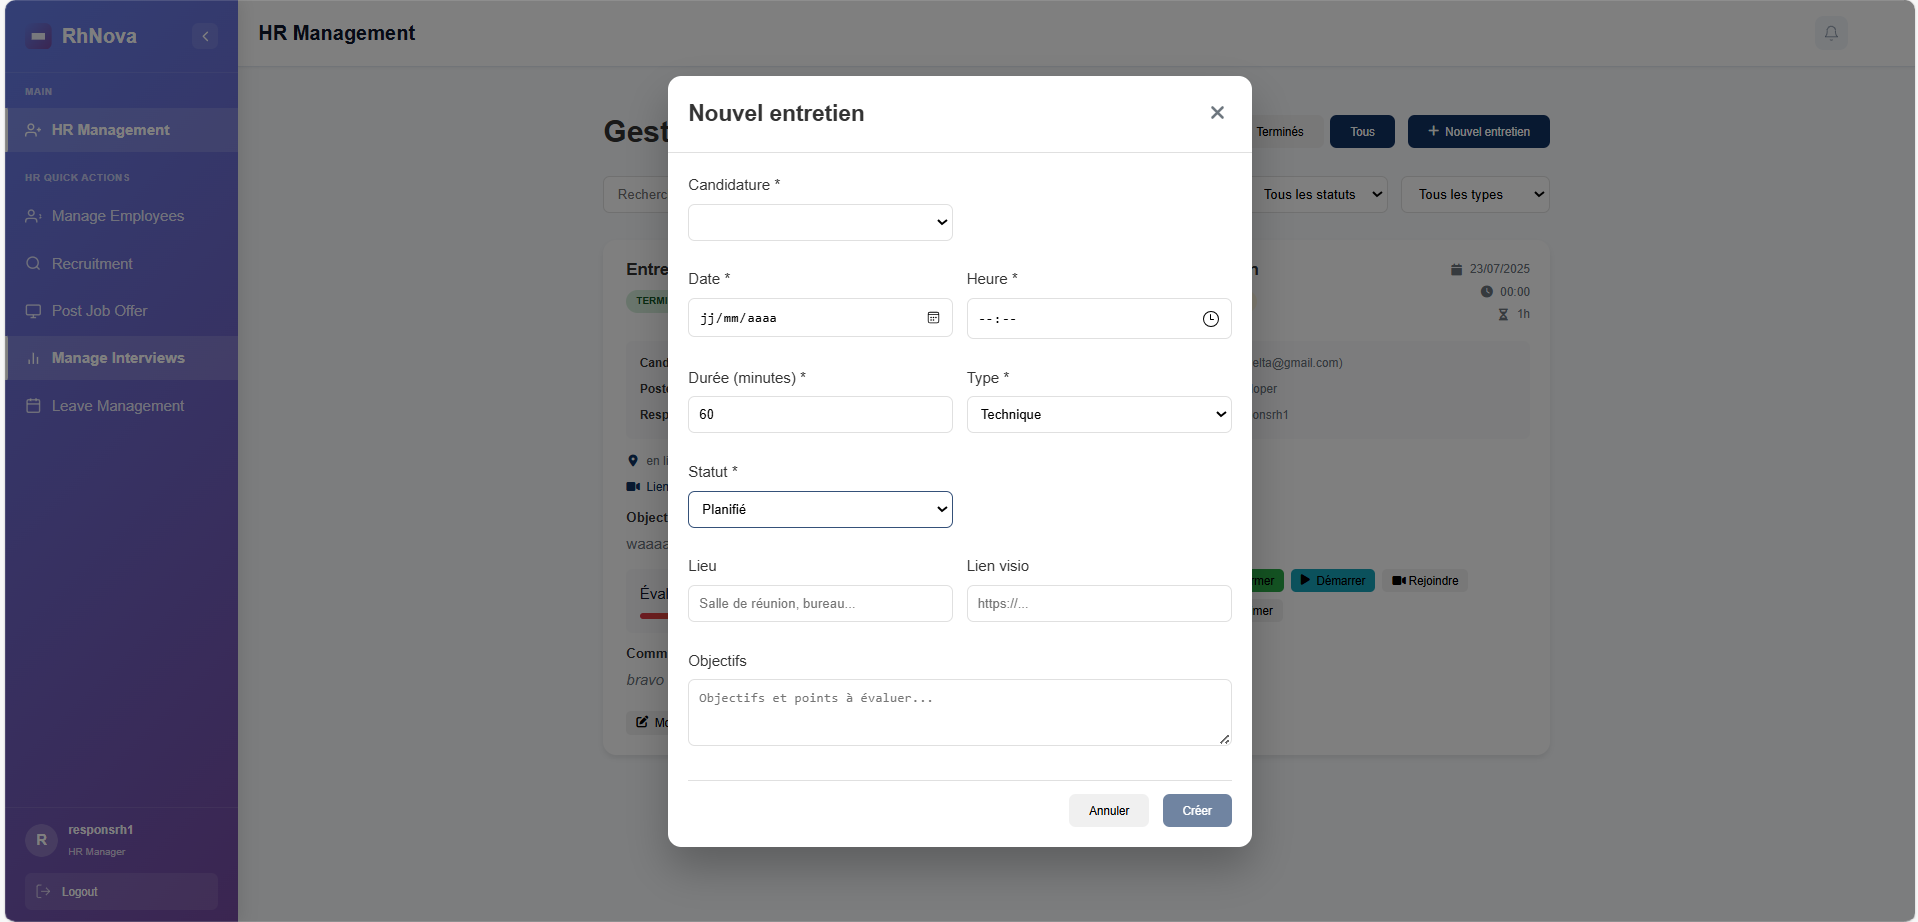
\includegraphics[width=\textwidth]{Figures/responsentretien.png}
             \caption{Liste des connecteurs}
         \end{figure}
     \end{itemize}
\end{itemize}

\section*{Conclusion}
En conclusion, ce chapitre a structuré la Sprint Gestion des Entretiens et ATS, en définissant les objectifs et détaillant le backlog, tout en exposant les diagrammes de cas d’utilisation, classes et de séquences. Les descriptions textuelles et captures d’écran ont confirmé la mise en œuvre réussie, établissant une base solide pour l’optimisation des processus de recrutement. Dans le chapitre suivant, nous aborderons les détails du quatrième  sprint " Gestion des Projets et Équipes".
\addcontentsline{toc}{section}{\protect\numberline{}Conclusion}%

